\documentclass{article}\usepackage[]{graphicx}\usepackage[]{color}
%% maxwidth is the original width if it is less than linewidth
%% otherwise use linewidth (to make sure the graphics do not exceed the margin)
\makeatletter
\def\maxwidth{ %
  \ifdim\Gin@nat@width>\linewidth
    \linewidth
  \else
    \Gin@nat@width
  \fi
}
\makeatother

\definecolor{fgcolor}{rgb}{0.345, 0.345, 0.345}
\newcommand{\hlnum}[1]{\textcolor[rgb]{0.686,0.059,0.569}{#1}}%
\newcommand{\hlstr}[1]{\textcolor[rgb]{0.192,0.494,0.8}{#1}}%
\newcommand{\hlcom}[1]{\textcolor[rgb]{0.678,0.584,0.686}{\textit{#1}}}%
\newcommand{\hlopt}[1]{\textcolor[rgb]{0,0,0}{#1}}%
\newcommand{\hlstd}[1]{\textcolor[rgb]{0.345,0.345,0.345}{#1}}%
\newcommand{\hlkwa}[1]{\textcolor[rgb]{0.161,0.373,0.58}{\textbf{#1}}}%
\newcommand{\hlkwb}[1]{\textcolor[rgb]{0.69,0.353,0.396}{#1}}%
\newcommand{\hlkwc}[1]{\textcolor[rgb]{0.333,0.667,0.333}{#1}}%
\newcommand{\hlkwd}[1]{\textcolor[rgb]{0.737,0.353,0.396}{\textbf{#1}}}%

\usepackage{framed}
\makeatletter
\newenvironment{kframe}{%
 \def\at@end@of@kframe{}%
 \ifinner\ifhmode%
  \def\at@end@of@kframe{\end{minipage}}%
  \begin{minipage}{\columnwidth}%
 \fi\fi%
 \def\FrameCommand##1{\hskip\@totalleftmargin \hskip-\fboxsep
 \colorbox{shadecolor}{##1}\hskip-\fboxsep
     % There is no \\@totalrightmargin, so:
     \hskip-\linewidth \hskip-\@totalleftmargin \hskip\columnwidth}%
 \MakeFramed {\advance\hsize-\width
   \@totalleftmargin\z@ \linewidth\hsize
   \@setminipage}}%
 {\par\unskip\endMakeFramed%
 \at@end@of@kframe}
\makeatother

\definecolor{shadecolor}{rgb}{.97, .97, .97}
\definecolor{messagecolor}{rgb}{0, 0, 0}
\definecolor{warningcolor}{rgb}{1, 0, 1}
\definecolor{errorcolor}{rgb}{1, 0, 0}
\newenvironment{knitrout}{}{} % an empty environment to be redefined in TeX

\usepackage{alltt}

\usepackage{textgreek}
\usepackage{hyperref}

\title{Worked Examples using \textsf{R}, \textit{Introductory Statistics, 7th ed.} by Neil Weiss}
\author{Charles Carter\thanks{cccarter@troy.edu}}
\date{October 1, 2014}
\IfFileExists{upquote.sty}{\usepackage{upquote}}{}
\begin{document}

\maketitle{}
\tableofcontents{}
\abstract{This paper consists of the worked examples in each chapter of \textit{Introductory Statistics, 7th Edition} by Neil Weiss, using the \textsf{R} programming language}

%chapter 1
\section{The Nature of Statistics}

%example 1.1
\subsection{Descriptive Statistics}This example contains no code.

%example 1.2
\subsection{Inferential Statistics}This example contains no code.

%example 1.3
\subsection{Classifying Statistical Studies}This example contains no code.

%example 1.4
\subsection{Classifying Statistical Studies}This example contains no code.

%example 1.5
\subsection{Simple Random Samples}

\begin{knitrout}
\definecolor{shadecolor}{rgb}{0.969, 0.969, 0.969}\color{fgcolor}\begin{kframe}
\begin{alltt}
\hlcom{#create vector of officials}
\hlkwd{library}\hlstd{(prob)}
\hlstd{off} \hlkwb{<-} \hlkwd{c}\hlstd{(}\hlstr{'G'}\hlstd{,} \hlstr{'L'}\hlstd{,} \hlstr{'S'}\hlstd{,} \hlstr{'A'}\hlstd{,} \hlstr{'T'}\hlstd{)}
\hlcom{#part a, list of samples of size 2}
\hlkwd{urnsamples}\hlstd{(off,} \hlnum{2}\hlstd{)}
\end{alltt}
\begin{verbatim}
##    X1 X2
## 1   G  L
## 2   G  S
## 3   G  A
## 4   G  T
## 5   L  S
## 6   L  A
## 7   L  T
## 8   S  A
## 9   S  T
## 10  A  T
\end{verbatim}
\begin{alltt}
\hlcom{#part d, list of samples of size 4}
\hlkwd{urnsamples}\hlstd{(off,} \hlnum{4}\hlstd{)}
\end{alltt}
\begin{verbatim}
##   X1 X2 X3 X4
## 1  G  L  S  A
## 2  G  L  S  T
## 3  G  L  A  T
## 4  G  S  A  T
## 5  L  S  A  T
\end{verbatim}
\end{kframe}
\end{knitrout}

%example 1.6
\subsection{Random-Number Tables}

\begin{knitrout}
\definecolor{shadecolor}{rgb}{0.969, 0.969, 0.969}\color{fgcolor}\begin{kframe}
\begin{alltt}
\hlcom{#generate 15 random integers between 1 and 728}
\hlkwd{sample}\hlstd{(}\hlnum{1}\hlopt{:}\hlnum{728}\hlstd{,} \hlnum{15}\hlstd{)}
\end{alltt}
\begin{verbatim}
##  [1] 418 204  25 556 649 355 149  80 479 245 129 462 325 259 383
\end{verbatim}
\end{kframe}
\end{knitrout}

%example 1.7
\subsection{Systematic Random Sampling}

\begin{knitrout}
\definecolor{shadecolor}{rgb}{0.969, 0.969, 0.969}\color{fgcolor}\begin{kframe}
\begin{alltt}
\hlcom{#declare variables}
\hlstd{pop} \hlkwb{<-} \hlnum{728}
\hlstd{sos} \hlkwb{<-} \hlnum{15}
\hlstd{division} \hlkwb{<-} \hlkwd{floor}\hlstd{(pop} \hlopt{/} \hlstd{sos)}
\hlstd{division}
\end{alltt}
\begin{verbatim}
## [1] 48
\end{verbatim}
\begin{alltt}
\hlstd{start} \hlkwb{<-} \hlkwd{sample}\hlstd{(}\hlnum{1}\hlopt{:}\hlstd{division,} \hlnum{1}\hlstd{)}
\hlstd{start}
\end{alltt}
\begin{verbatim}
## [1] 8
\end{verbatim}
\begin{alltt}
\hlcom{#generate sequence}
\hlstd{s} \hlkwb{<-} \hlkwd{seq}\hlstd{(start, pop, division)}
\hlstd{s}
\end{alltt}
\begin{verbatim}
##  [1]   8  56 104 152 200 248 296 344 392 440 488 536 584 632 680 728
\end{verbatim}
\end{kframe}
\end{knitrout}

%example 1.8
\subsection{}

%example 1.9
\subsection{}

%example 1.10
\subsection{}

%example 1.11
\subsection{}

%example 1.12
\subsection{}

%example 1.13
\subsection{}

%chapter 2
\section{Organizing Data}

%example 2.1
\subsection{Variables and Data}This example contains no code.

%example 2.2
\subsection{Variables and Data}This example contains no code.

%example 2.3
\subsection{Variables and Data}This example contains no code.

%example 2.4
\subsection{Variables and Data}This example contains no code.

%example 2.5
\subsection{Grouping Quantitative Data}

\begin{knitrout}
\definecolor{shadecolor}{rgb}{0.969, 0.969, 0.969}\color{fgcolor}\begin{kframe}
\begin{alltt}
\hlcom{#read in the data}
\hlstd{invest} \hlkwb{<-} \hlkwd{read.csv}\hlstd{(}\hlstr{"data/Tb02-01.txt"}\hlstd{)}
\hlkwd{str}\hlstd{(invest)}
\end{alltt}
\begin{verbatim}
## 'data.frame':	40 obs. of  1 variable:
##  $ DAYS: int  70 64 99 55 64 89 87 65 62 38 ...
\end{verbatim}
\begin{alltt}
\hlstd{w} \hlkwb{<-} \hlkwd{cut}\hlstd{(invest}\hlopt{$}\hlstd{DAYS,} \hlkwd{c}\hlstd{(}\hlnum{30}\hlstd{,} \hlnum{40}\hlstd{,} \hlnum{50}\hlstd{,} \hlnum{60}\hlstd{,} \hlnum{70}\hlstd{,} \hlnum{80}\hlstd{,} \hlnum{90}\hlstd{,} \hlnum{100}\hlstd{),} \hlkwc{right} \hlstd{=} \hlnum{FALSE}\hlstd{)}
\hlstd{invest}\hlopt{$}\hlstd{CAT} \hlkwb{<-} \hlstd{w}
\hlkwd{table}\hlstd{(invest}\hlopt{$}\hlstd{CAT)}
\end{alltt}
\begin{verbatim}
## 
##  [30,40)  [40,50)  [50,60)  [60,70)  [70,80)  [80,90) [90,100) 
##        3        1        8       10        7        7        4
\end{verbatim}
\begin{alltt}
\hlstd{x} \hlkwb{<-} \hlkwd{table}\hlstd{(invest}\hlopt{$}\hlstd{CAT)}
\hlstd{y} \hlkwb{<-} \hlkwd{prop.table}\hlstd{(x)}
\hlstd{z} \hlkwb{<-}  \hlkwd{merge}\hlstd{(x, y,} \hlkwc{by.x} \hlstd{=} \hlstr{"Var1"}\hlstd{,} \hlkwc{by.y} \hlstd{=} \hlstr{"Var1"}\hlstd{)}
\hlstd{z}
\end{alltt}
\begin{verbatim}
##       Var1 Freq.x Freq.y
## 1  [30,40)      3  0.075
## 2  [40,50)      1  0.025
## 3  [50,60)      8  0.200
## 4  [60,70)     10  0.250
## 5  [70,80)      7  0.175
## 6  [80,90)      7  0.175
## 7 [90,100)      4  0.100
\end{verbatim}
\end{kframe}
\end{knitrout}


%example 2.6
\subsection{}

%example 2.7
\subsection{}

%example 2.8
\subsection{}

%example 2.9
\subsection{}

%example 2.10
\subsection{}

%example 2.11
\subsection{}

%example 2.12
\subsection{}

%example 2.13
\subsection{}

%example 2.14
\subsection{}

%example 2.15
\subsection{}

%example 2.16
\subsection{}

%example 2.17
\subsection{}

%example 2.18
\subsection{}

%chapter 3
\section{Descriptive Measures}



%chapter 4
\section{Probability Concepts}


%chapter 5
\section{Discrete Random Variables}


%chapter 6
\section{The Normal Distribution}

\subsection{Example 6.1,}
\subsection{Example 6.2,}
\subsection{Example 6.3,}
\subsection{Example 6.4,}
\subsection{Example 6.5,}
\subsection{Example 6.6,}
\subsection{Example 6.7,}
\subsection{Example 6.8,}
\subsection{Example 6.9,}
\subsection{Example 6.10,}
\subsection{Example 6.11,}
\subsection{Example 6.12,}

\subsection{Example 6.13, Using Technology to Obtain Normal Percentiles}
\begin{knitrout}
\definecolor{shadecolor}{rgb}{0.969, 0.969, 0.969}\color{fgcolor}\begin{kframe}
\begin{alltt}
\hlstd{mu} \hlkwb{<-} \hlnum{100}
\hlstd{sigma} \hlkwb{<-} \hlnum{16}
\hlstd{ptile} \hlkwb{<-} \hlkwd{qnorm}\hlstd{(}\hlnum{0.90}\hlstd{, mu, sigma)}
\hlstd{ptile}
\end{alltt}
\begin{verbatim}
## [1] 120.5
\end{verbatim}
\end{kframe}
\end{knitrout}

\subsection{Example 6.14, Normal Probability Plots}
\begin{knitrout}
\definecolor{shadecolor}{rgb}{0.969, 0.969, 0.969}\color{fgcolor}\begin{kframe}
\begin{alltt}
\hlcom{#read in the data}
\hlstd{income} \hlkwb{<-} \hlkwd{read.csv}\hlstd{(}\hlstr{"data/Tb06-03.txt"}\hlstd{)}
\hlkwd{str}\hlstd{(income)}
\end{alltt}
\begin{verbatim}
## 'data.frame':	12 obs. of  1 variable:
##  $ AGI: num  9.7 93.1 33 21.2 81.4 51.1 43.5 10.6 12.8 7.8 ...
\end{verbatim}
\begin{alltt}
\hlkwd{qqnorm}\hlstd{(income}\hlopt{$}\hlstd{AGI,} \hlkwc{datax} \hlstd{=} \hlnum{TRUE}\hlstd{)}
\end{alltt}
\end{kframe}
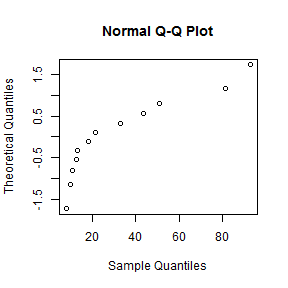
\includegraphics[width=\maxwidth]{figure/ex06-14} 

\end{knitrout}

%chapter 7
\section{The Sampling Distribution of the Sample Mean}


%chapter 8
\section{Confidence Intervals for One Population Mean}

\subsection{Example 8.1, Estimating a Population Mean}
\begin{knitrout}
\definecolor{shadecolor}{rgb}{0.969, 0.969, 0.969}\color{fgcolor}\begin{kframe}
\begin{alltt}
\hlcom{#read in the data}
\hlstd{prices} \hlkwb{<-} \hlkwd{read.csv}\hlstd{(}\hlstr{"data/Tb08-01.txt"}\hlstd{)}
\hlkwd{str}\hlstd{(prices)}
\end{alltt}
\begin{verbatim}
## 'data.frame':	36 obs. of  1 variable:
##  $ PRICE: num  53.8 54.4 45.2 42.9 49.9 48.2 41.6 58.9 48.6 53.1 ...
\end{verbatim}
\begin{alltt}
\hlkwd{hist}\hlstd{(prices}\hlopt{$}\hlstd{PRICE,} \hlkwc{breaks} \hlstd{=} \hlnum{5}\hlstd{)}
\end{alltt}
\end{kframe}
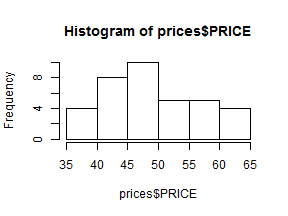
\includegraphics[width=\maxwidth]{figure/ex08-01} 
\begin{kframe}\begin{alltt}
\hlstd{sum} \hlkwb{<-} \hlkwd{sum}\hlstd{(prices}\hlopt{$}\hlstd{PRICE)}
\hlstd{n} \hlkwb{<-} \hlkwd{nrow}\hlstd{(prices)}
\hlstd{mu} \hlkwb{<-} \hlstd{sum} \hlopt{/} \hlstd{n}
\hlcom{#alternatively}
\hlstd{mu1} \hlkwb{<-} \hlkwd{mean}\hlstd{(prices}\hlopt{$}\hlstd{PRICE)}
\end{alltt}
\end{kframe}
\end{knitrout}

\paragraph{}The estimated population, $\mu$, from the sample mean, $\bar{x}$, is 49.2778.

\subsection{Example 8.2, Introducing Confidence Intervals}
\begin{knitrout}
\definecolor{shadecolor}{rgb}{0.969, 0.969, 0.969}\color{fgcolor}\begin{kframe}
\begin{alltt}
\hlcom{#read in the data}
\hlstd{prices} \hlkwb{<-} \hlkwd{read.csv}\hlstd{(}\hlstr{"data/Tb08-01.txt"}\hlstd{)}
\hlkwd{str}\hlstd{(prices)}
\end{alltt}
\begin{verbatim}
## 'data.frame':	36 obs. of  1 variable:
##  $ PRICE: num  53.8 54.4 45.2 42.9 49.9 48.2 41.6 58.9 48.6 53.1 ...
\end{verbatim}
\begin{alltt}
\hlkwd{hist}\hlstd{(prices}\hlopt{$}\hlstd{PRICE,} \hlkwc{breaks} \hlstd{=} \hlnum{5}\hlstd{)}
\end{alltt}
\end{kframe}
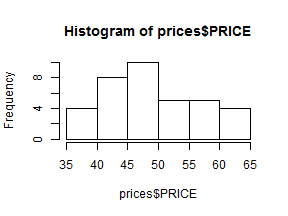
\includegraphics[width=\maxwidth]{figure/ex08-02} 
\begin{kframe}\begin{alltt}
\hlstd{sum} \hlkwb{<-} \hlkwd{sum}\hlstd{(prices}\hlopt{$}\hlstd{PRICE)}
\hlstd{n} \hlkwb{<-} \hlkwd{nrow}\hlstd{(prices)}
\hlstd{mu} \hlkwb{<-} \hlstd{sum} \hlopt{/} \hlstd{n}
\hlstd{sigma} \hlkwb{<-} \hlnum{7.2}
\hlstd{s} \hlkwb{<-} \hlstd{sigma} \hlopt{/} \hlkwd{sqrt}\hlstd{(n)}
\hlkwd{cat}\hlstd{(sum, n, mu, sigma, s)}
\end{alltt}
\begin{verbatim}
## 1774 36 49.28 7.2 1.2
\end{verbatim}
\begin{alltt}
\hlstd{confidence.interval} \hlkwb{<-} \hlkwd{simple.z.test}\hlstd{(prices}\hlopt{$}\hlstd{PRICE, sigma,} \hlkwc{conf.level} \hlstd{=} \hlnum{0.9544}\hlstd{)}
\hlstd{confidence.interval}
\end{alltt}
\begin{verbatim}
## [1] 46.88 51.68
\end{verbatim}
\end{kframe}
\end{knitrout}

\subsection{Example 8.3, Interpreting Confidence Intervals}

\subsection{Example 8.4, The One-Sample z-Interval Procedure}
\subsection{Example 8.5, Using Technology to Obtain a z-Interval}
\subsection{Example 8.6, Introducing the Margin of Error}
\subsection{Example 8.7, Sample Size for Estimating $\mu{}$}
\subsection{Example 8.8, Finding the t-Value Having a Specified Area to the Right}
\subsection{Example 8.9, The One-Sample t-Interval Procedure}
\subsection{Example 8.10, The One-Sample t-Interval Procedure}
\subsection{Example 8.11, Choosing a Confidence Interval Procedure}

%chapter 9
\section{Hypothesis Tests for One Population Mean}

\subsection{Example 9.1, Choosing the Null and Alternative Hypotheses}This example contains no code.
\subsection{Example 9.2, Choosing the Null and Alternative Hypotheses}This example contains no code.
\subsection{Example 9.3, Choosing the Null and Alternative Hypotheses}This example contains no code.
\subsection{Example 9.4, The Logic of Hypothesis Testing}

Null hypothesis is $H_0: \mu = 454$. \\
Alternative hypothesis is $H_\alpha: \mu \not= 454$.

\begin{knitrout}
\definecolor{shadecolor}{rgb}{0.969, 0.969, 0.969}\color{fgcolor}\begin{kframe}
\begin{alltt}
\hlcom{# load the data file}
\hlstd{weights} \hlkwb{<-} \hlkwd{read.csv}\hlstd{(}\hlstr{"data/Tb09-01.txt"}\hlstd{)}
\hlkwd{str}\hlstd{(weights)}
\end{alltt}
\begin{verbatim}
## 'data.frame':	25 obs. of  1 variable:
##  $ WEIGHT: int  465 456 438 454 447 449 442 449 446 447 ...
\end{verbatim}
\begin{alltt}
\hlcom{#declare and initialize variables}
\hlstd{mu} \hlkwb{<-} \hlnum{454}
\hlstd{sigma} \hlkwb{<-} \hlnum{7.8}
\hlstd{n} \hlkwb{<-} \hlnum{25}
\hlstd{xbar} \hlkwb{<-} \hlkwd{mean}\hlstd{(weights}\hlopt{$}\hlstd{WEIGHT)}
\hlstd{ztest} \hlkwb{<-} \hlstd{(xbar} \hlopt{-} \hlstd{mu)} \hlopt{/} \hlstd{(sigma} \hlopt{/} \hlkwd{sqrt}\hlstd{(n))}
\hlstd{ztest}
\end{alltt}
\begin{verbatim}
## [1] -2.564
\end{verbatim}
\begin{alltt}
\hlcom{#determine the result of the test}
\hlstd{result} \hlkwb{<-} \hlkwd{pnorm}\hlstd{(ztest)}
\hlstd{result}
\end{alltt}
\begin{verbatim}
## [1] 0.005172
\end{verbatim}
\begin{alltt}
\hlcom{#use simple z test from UsingR package}
\hlkwd{library}\hlstd{(UsingR)}
\hlstd{conf.int} \hlkwb{<-} \hlkwd{simple.z.test}\hlstd{(weights}\hlopt{$}\hlstd{WEIGHT,} \hlkwc{sigma} \hlstd{= sigma,} \hlkwc{conf.level} \hlstd{=} \hlnum{0.9544}\hlstd{)}
\hlstd{conf.int}
\end{alltt}
\begin{verbatim}
## [1] 446.9 453.1
\end{verbatim}
\end{kframe}
\end{knitrout}

\paragraph{}The claimed weight of the population is $\mu{}$ per bag, $454$ grams. The mean sample weight is $\bar{x}$ per bag, $450$ grams. The $z$ value is $\ensuremath{-2.5641}$, which is more than two standard deviations below the population mean. 


\subsection{Example 9.5, Type I and Type II Errors}This example contains no code.
\subsection{Example 9.6, Obtaining the Critical Values}

\begin{knitrout}
\definecolor{shadecolor}{rgb}{0.969, 0.969, 0.969}\color{fgcolor}\begin{kframe}
\begin{alltt}
\hlstd{left.tail} \hlkwb{<-} \hlkwd{qnorm}\hlstd{(}\hlnum{0.05}\hlstd{)}
\hlstd{left.tail}
\end{alltt}
\begin{verbatim}
## [1] -1.645
\end{verbatim}
\begin{alltt}
\hlstd{right.tail} \hlkwb{<-} \hlkwd{qnorm}\hlstd{(}\hlnum{0.95}\hlstd{)}
\hlstd{right.tail}
\end{alltt}
\begin{verbatim}
## [1] 1.645
\end{verbatim}
\begin{alltt}
\hlstd{two.tail.left} \hlkwb{<-} \hlkwd{qnorm}\hlstd{(}\hlnum{0.025}\hlstd{)}
\hlstd{two.tail.left}
\end{alltt}
\begin{verbatim}
## [1] -1.96
\end{verbatim}
\begin{alltt}
\hlstd{two.tail.right} \hlkwb{<-} \hlkwd{qnorm}\hlstd{(}\hlnum{0.975}\hlstd{)}
\hlstd{two.tail.right}
\end{alltt}
\begin{verbatim}
## [1] 1.96
\end{verbatim}
\end{kframe}
\end{knitrout}

\subsection{Example 9.7, The One-Sample z-Test}

Null hypothesis is $H_0: \mu = \$51.46$. \\
Alternative hypothesis is $H_\alpha: > \$51.46$

\begin{knitrout}
\definecolor{shadecolor}{rgb}{0.969, 0.969, 0.969}\color{fgcolor}\begin{kframe}
\begin{alltt}
\hlcom{# load the data file}
\hlstd{books} \hlkwb{<-} \hlkwd{read.csv}\hlstd{(}\hlstr{"data/Tb09-05.txt"}\hlstd{)}
\hlkwd{str}\hlstd{(books)}
\end{alltt}
\begin{verbatim}
## 'data.frame':	40 obs. of  1 variable:
##  $ PRICE: num  56 46.2 47.3 54 53.7 ...
\end{verbatim}
\begin{alltt}
\hlcom{#declare and initialize variables}
\hlstd{mu} \hlkwb{<-} \hlnum{51.46}
\hlstd{sigma} \hlkwb{<-} \hlnum{7.61}
\hlstd{n} \hlkwb{<-} \hlnum{40}
\hlstd{xbar} \hlkwb{<-} \hlkwd{mean}\hlstd{(books}\hlopt{$}\hlstd{PRICE)}
\hlstd{right.tail} \hlkwb{=} \hlnum{0.01}
\hlstd{ztest} \hlkwb{<-} \hlstd{(xbar} \hlopt{-} \hlstd{mu)} \hlopt{/} \hlstd{(sigma} \hlopt{/} \hlkwd{sqrt}\hlstd{(n))}
\hlstd{ztest}
\end{alltt}
\begin{verbatim}
## [1] 2.851
\end{verbatim}
\begin{alltt}
\hlstd{right.crit} \hlkwb{<-} \hlkwd{qnorm}\hlstd{(}\hlnum{1} \hlopt{-} \hlstd{right.tail)}
\hlstd{right.crit}
\end{alltt}
\begin{verbatim}
## [1] 2.326
\end{verbatim}
\end{kframe}
\end{knitrout}

\paragraph{}The $z$ statistic is 2.8508, which is greater than the critical value of 2.3263, so we reject the null hypothesis.

\subsection{Example 9.8, The One-Sample z-Test}

Null hypothesis is $H_0: \mu = 800$. \\
Alternative hypothesis is $H_\alpha: < 800$

\begin{knitrout}
\definecolor{shadecolor}{rgb}{0.969, 0.969, 0.969}\color{fgcolor}\begin{kframe}
\begin{alltt}
\hlcom{# load the data file}
\hlstd{rda} \hlkwb{<-} \hlkwd{read.csv}\hlstd{(}\hlstr{"data/Tb09-06.txt"}\hlstd{)}
\hlkwd{str}\hlstd{(rda)}
\end{alltt}
\begin{verbatim}
## 'data.frame':	18 obs. of  1 variable:
##  $ CALCI: int  686 433 743 647 734 641 993 620 574 634 ...
\end{verbatim}
\begin{alltt}
\hlcom{#declare and initialize variables}
\hlstd{mu} \hlkwb{<-} \hlnum{800}
\hlstd{sigma} \hlkwb{<-} \hlnum{188}
\hlstd{n} \hlkwb{<-} \hlnum{18}
\hlstd{xbar} \hlkwb{<-} \hlkwd{mean}\hlstd{(rda}\hlopt{$}\hlstd{CALCI)}
\hlstd{left.tail} \hlkwb{=} \hlnum{0.05}
\hlstd{ztest} \hlkwb{<-} \hlstd{(xbar} \hlopt{-} \hlstd{mu)} \hlopt{/} \hlstd{(sigma} \hlopt{/} \hlkwd{sqrt}\hlstd{(n))}
\hlstd{ztest}
\end{alltt}
\begin{verbatim}
## [1] -1.187
\end{verbatim}
\begin{alltt}
\hlstd{left.crit} \hlkwb{<-} \hlkwd{qnorm}\hlstd{(left.tail)}
\hlstd{left.crit}
\end{alltt}
\begin{verbatim}
## [1] -1.645
\end{verbatim}
\end{kframe}
\end{knitrout}

\paragraph{}The $z$ statistic is \ensuremath{-1.1873}, which is less than the critical value of \ensuremath{-1.6449}, so we do not reject the null hypothesis.

\subsection{Example 9.9, The One-Sample z-Test}

Null hypothesis is $H_0: \mu = 60$. \\
Alternative hypothesis is $H_\alpha: \not= 60$

\begin{knitrout}
\definecolor{shadecolor}{rgb}{0.969, 0.969, 0.969}\color{fgcolor}\begin{kframe}
\begin{alltt}
\hlcom{# load the data file}
\hlstd{cheetah} \hlkwb{<-} \hlkwd{read.csv}\hlstd{(}\hlstr{"data/Tb09-07.txt"}\hlstd{)}
\hlkwd{str}\hlstd{(cheetah)}
\end{alltt}
\begin{verbatim}
## 'data.frame':	35 obs. of  1 variable:
##  $ SPEEDS: num  57.3 57.5 59 56.5 61.3 57.6 59.2 65 60.1 59.7 ...
\end{verbatim}
\begin{alltt}
\hlcom{#histogram of the data set}
\hlkwd{hist}\hlstd{(cheetah}\hlopt{$}\hlstd{SPEEDS,} \hlkwc{breaks} \hlstd{=} \hlnum{15}\hlstd{,} \hlkwc{xlab} \hlstd{=} \hlstr{"Cheetah Speeds"}\hlstd{,} \hlkwc{ylab} \hlstd{=} \hlstr{"Counts"}\hlstd{,} \hlkwc{main} \hlstd{=} \hlstr{"Histogram of Cheetah Speeds Sample"}\hlstd{)}
\end{alltt}
\end{kframe}
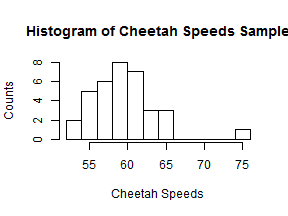
\includegraphics[width=\maxwidth]{figure/ex09-09} 
\begin{kframe}\begin{alltt}
\hlcom{#declare and initialize variables}
\hlstd{mu} \hlkwb{<-} \hlnum{60}
\hlstd{sigma} \hlkwb{<-} \hlnum{3.2}
\hlstd{n} \hlkwb{<-} \hlnum{35}
\hlstd{xbar} \hlkwb{<-} \hlkwd{mean}\hlstd{(cheetah}\hlopt{$}\hlstd{SPEEDS)}
\hlstd{tails} \hlkwb{=} \hlnum{0.05}
\hlstd{ztest} \hlkwb{<-} \hlstd{(xbar} \hlopt{-} \hlstd{mu)} \hlopt{/} \hlstd{(sigma} \hlopt{/} \hlkwd{sqrt}\hlstd{(n))}
\hlstd{ztest}
\end{alltt}
\begin{verbatim}
## [1] -0.8768
\end{verbatim}
\begin{alltt}
\hlstd{crits} \hlkwb{<-} \hlkwd{qnorm}\hlstd{(}\hlkwd{c}\hlstd{( tails} \hlopt{/} \hlnum{2}\hlstd{, (}\hlnum{1} \hlopt{-} \hlstd{tails} \hlopt{/} \hlnum{2}\hlstd{)))}
\hlstd{crits}
\end{alltt}
\begin{verbatim}
## [1] -1.96  1.96
\end{verbatim}
\end{kframe}
\end{knitrout}

\paragraph{}The $z$ statistic is \ensuremath{-0.8768}, which is less than the critical values of \ensuremath{-1.96}, 1.96, so we do not reject the null hypothesis.

\subsection{Example 9.10, }
\subsection{Example 9.11, }
\subsection{Example 9.12, }
\subsection{Example 9.13, }
\subsection{Example 9.14, }
\subsection{Example 9.15, }
\subsection{Example 9.16, }
\subsection{Example 9.17, }
\subsection{Example 9.18, }
\subsection{Example 9.19, }
\subsection{Example 9.20, }
\subsection{Example 9.21, }

%chapter 10
\section{Inferences for Two Population Means}
%chapter 11
\section{Inferences for Population Standard Deviations}
%chapter 12
\section{Inferences for Population Proportions}
%chapter 13
\section{Chi-Square Procedures}
%chapter 14
\section{Descriptive Methods in Regression and Correlation}

%Example 14.1
\subsection{Linear Equations}
\begin{knitrout}
\definecolor{shadecolor}{rgb}{0.969, 0.969, 0.969}\color{fgcolor}\begin{kframe}
\begin{alltt}
\hlcom{# load the data file}
\hlstd{wp} \hlkwb{<-} \hlkwd{read.csv}\hlstd{(}\hlstr{"data/Tb14-01.txt"}\hlstd{,} \hlkwc{sep} \hlstd{=} \hlstr{"\textbackslash{}t"}\hlstd{)}
\hlkwd{str}\hlstd{(wp)}
\end{alltt}
\begin{verbatim}
## 'data.frame':	5 obs. of  2 variables:
##  $ TIME: num  5 7.5 15 20 22.5
##  $ COST: int  125 175 325 425 475
\end{verbatim}
\begin{alltt}
\hlstd{x} \hlkwb{<-} \hlstd{wp}\hlopt{$}\hlstd{TIME}
\hlstd{y} \hlkwb{<-} \hlnum{25} \hlopt{+} \hlstd{(}\hlnum{20} \hlopt{*} \hlstd{x)}
\hlstd{line} \hlkwb{<-} \hlkwd{lm}\hlstd{(y} \hlopt{~} \hlstd{x)}
\hlkwd{plot}\hlstd{(x, y,} \hlkwc{xlim} \hlstd{=} \hlkwd{c}\hlstd{(}\hlnum{0}\hlstd{,}\hlnum{25}\hlstd{),} \hlkwc{ylim} \hlstd{=} \hlkwd{c}\hlstd{(}\hlnum{0}\hlstd{,}\hlnum{500}\hlstd{))}
\hlkwd{abline}\hlstd{(line)}
\end{alltt}
\end{kframe}
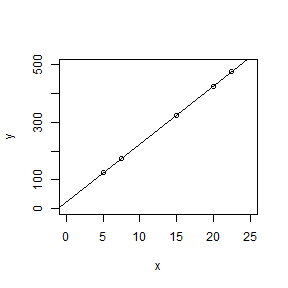
\includegraphics[width=\maxwidth]{figure/ex14-01} 

\end{knitrout}

%example 14.2
\subsection{y-Intercept and Slope}
\begin{knitrout}
\definecolor{shadecolor}{rgb}{0.969, 0.969, 0.969}\color{fgcolor}\begin{kframe}
\begin{alltt}
\hlcom{# load dummy data}
\hlstd{x} \hlkwb{<-} \hlkwd{c}\hlstd{(}\hlopt{-}\hlnum{1}\hlopt{:}\hlnum{10}\hlstd{)}
\hlstd{y} \hlkwb{<-} \hlnum{25} \hlopt{+} \hlstd{(}\hlnum{20} \hlopt{*} \hlstd{x)}
\hlstd{line} \hlkwb{<-} \hlkwd{lm}\hlstd{(y} \hlopt{~} \hlstd{x)}
\hlkwd{plot}\hlstd{(x, y,} \hlkwc{xlim} \hlstd{=} \hlkwd{c}\hlstd{(}\hlopt{-}\hlnum{1}\hlstd{,}\hlnum{10}\hlstd{),} \hlkwc{ylim} \hlstd{=} \hlkwd{c}\hlstd{(}\hlopt{-}\hlnum{50}\hlstd{,}\hlnum{200}\hlstd{))}
\hlkwd{abline}\hlstd{(line)}
\hlkwd{abline}\hlstd{(}\hlkwc{v}\hlstd{=}\hlnum{0}\hlstd{,}\hlkwc{col}\hlstd{=}\hlstr{"red"}\hlstd{,} \hlkwc{lty} \hlstd{=} \hlnum{2}\hlstd{)}
\hlkwd{abline}\hlstd{(}\hlkwc{h}\hlstd{=}\hlnum{0}\hlstd{,}\hlkwc{col}\hlstd{=}\hlstr{"red"}\hlstd{,} \hlkwc{lty} \hlstd{=} \hlnum{3}\hlstd{)}
\end{alltt}
\end{kframe}
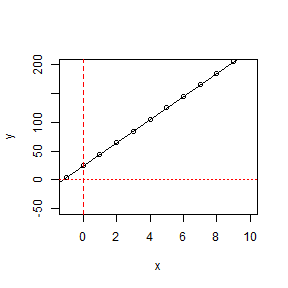
\includegraphics[width=\maxwidth]{figure/ex14-02} 

\end{knitrout}

%example 14.3
\subsection{Introducing the Least Squares Criterion}

\begin{knitrout}
\definecolor{shadecolor}{rgb}{0.969, 0.969, 0.969}\color{fgcolor}\begin{kframe}
\begin{alltt}
\hlstd{x} \hlkwb{<-} \hlkwd{c}\hlstd{(}\hlnum{1}\hlstd{,}\hlnum{1}\hlstd{,}\hlnum{2}\hlstd{,}\hlnum{4}\hlstd{)}
\hlstd{y} \hlkwb{<-} \hlkwd{c}\hlstd{(}\hlnum{1}\hlstd{,}\hlnum{2}\hlstd{,}\hlnum{2}\hlstd{,}\hlnum{6}\hlstd{)}
\hlstd{df} \hlkwb{<-} \hlkwd{data.frame}\hlstd{(x,y)}
\hlstd{df}
\end{alltt}
\begin{verbatim}
##   x y
## 1 1 1
## 2 1 2
## 3 2 2
## 4 4 6
\end{verbatim}
\begin{alltt}
\hlkwd{plot}\hlstd{(df,} \hlkwc{xlim} \hlstd{=} \hlkwd{c}\hlstd{(}\hlnum{0}\hlstd{,} \hlnum{4}\hlstd{),} \hlkwc{ylim} \hlstd{=} \hlkwd{c}\hlstd{(}\hlnum{0}\hlstd{,} \hlnum{6}\hlstd{))}
\hlstd{line} \hlkwb{<-} \hlkwd{lm}\hlstd{(y} \hlopt{~} \hlstd{x)}
\hlstd{line}
\end{alltt}
\begin{verbatim}
## 
## Call:
## lm(formula = y ~ x)
## 
## Coefficients:
## (Intercept)            x  
##       -0.25         1.50
\end{verbatim}
\begin{alltt}
\hlkwd{abline}\hlstd{(line)}
\end{alltt}
\end{kframe}
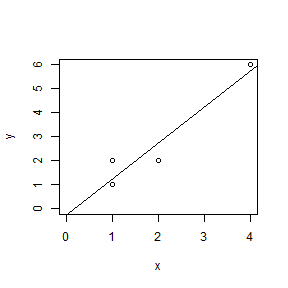
\includegraphics[width=\maxwidth]{figure/ex14-03} 

\end{knitrout}

%example 14.4
\subsection{The Regression Equation}

\begin{knitrout}
\definecolor{shadecolor}{rgb}{0.969, 0.969, 0.969}\color{fgcolor}\begin{kframe}
\begin{alltt}
\hlcom{# load Orion data}
\hlstd{orion} \hlkwb{<-} \hlkwd{read.csv}\hlstd{(}\hlstr{"data/Tb14-02.txt"}\hlstd{,} \hlkwc{sep} \hlstd{=} \hlstr{"\textbackslash{}t"}\hlstd{)}
\hlkwd{str}\hlstd{(orion)}
\end{alltt}
\begin{verbatim}
## 'data.frame':	11 obs. of  2 variables:
##  $ AGE  : int  5 4 6 5 5 5 6 6 2 7 ...
##  $ PRICE: int  85 103 70 82 89 98 66 95 169 70 ...
\end{verbatim}
\begin{alltt}
\hlstd{s} \hlkwb{<-} \hlkwd{lm}\hlstd{(orion}\hlopt{$}\hlstd{PRICE} \hlopt{~} \hlstd{orion}\hlopt{$}\hlstd{AGE)}
\hlstd{s}
\end{alltt}
\begin{verbatim}
## 
## Call:
## lm(formula = orion$PRICE ~ orion$AGE)
## 
## Coefficients:
## (Intercept)    orion$AGE  
##       195.5        -20.3
\end{verbatim}
\begin{alltt}
\hlkwd{plot}\hlstd{(orion}\hlopt{$}\hlstd{AGE, orion}\hlopt{$}\hlstd{PRICE)}
\hlkwd{abline}\hlstd{(s)}
\end{alltt}
\end{kframe}
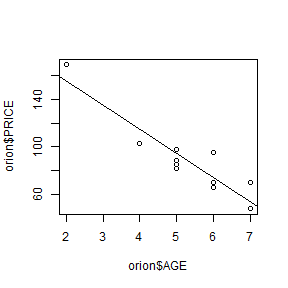
\includegraphics[width=\maxwidth]{figure/ex14-04} 
\begin{kframe}\begin{alltt}
\hlcom{# find y for x equals 3 and 4}
\hlstd{s}\hlopt{$}\hlstd{coefficients}
\end{alltt}
\begin{verbatim}
## (Intercept)   orion$AGE 
##      195.47      -20.26
\end{verbatim}
\begin{alltt}
\hlstd{intercept} \hlkwb{<-} \hlstd{s}\hlopt{$}\hlstd{coefficients[[}\hlnum{1}\hlstd{]]}
\hlstd{slope} \hlkwb{<-} \hlstd{s}\hlopt{$}\hlstd{coefficients[[}\hlnum{2}\hlstd{]]}
\hlstd{three.year.old.Orion} \hlkwb{<-} \hlstd{intercept} \hlopt{+} \hlstd{( slope} \hlopt{*} \hlnum{3}\hlstd{)}
\hlstd{three.year.old.Orion}
\end{alltt}
\begin{verbatim}
## [1] 134.7
\end{verbatim}
\begin{alltt}
\hlstd{four.year.old.Orion} \hlkwb{<-} \hlstd{intercept} \hlopt{+} \hlstd{( slope} \hlopt{*} \hlnum{4}\hlstd{)}
\hlstd{four.year.old.Orion}
\end{alltt}
\begin{verbatim}
## [1] 114.4
\end{verbatim}
\end{kframe}
\end{knitrout}

%example 14.5
\subsection{Using Technology to Obtain a Scatter Diagram}

\begin{knitrout}
\definecolor{shadecolor}{rgb}{0.969, 0.969, 0.969}\color{fgcolor}\begin{kframe}
\begin{alltt}
\hlcom{# load Orion data}
\hlstd{orion} \hlkwb{<-} \hlkwd{read.csv}\hlstd{(}\hlstr{"data/Tb14-02.txt"}\hlstd{,} \hlkwc{sep} \hlstd{=} \hlstr{"\textbackslash{}t"}\hlstd{)}
\hlkwd{str}\hlstd{(orion)}
\end{alltt}
\begin{verbatim}
## 'data.frame':	11 obs. of  2 variables:
##  $ AGE  : int  5 4 6 5 5 5 6 6 2 7 ...
##  $ PRICE: int  85 103 70 82 89 98 66 95 169 70 ...
\end{verbatim}
\begin{alltt}
\hlkwd{plot}\hlstd{(orion}\hlopt{$}\hlstd{AGE, orion}\hlopt{$}\hlstd{PRICE)}
\end{alltt}
\end{kframe}
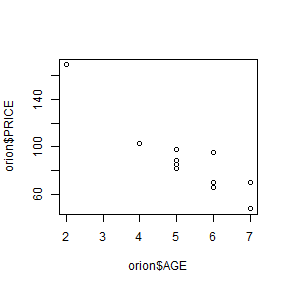
\includegraphics[width=\maxwidth]{figure/ex14-05} 

\end{knitrout}

%example 14.6
\subsection{Using Technology to Obtain a Regression Line}

\begin{knitrout}
\definecolor{shadecolor}{rgb}{0.969, 0.969, 0.969}\color{fgcolor}\begin{kframe}
\begin{alltt}
\hlcom{# load Orion data}
\hlstd{orion} \hlkwb{<-} \hlkwd{read.csv}\hlstd{(}\hlstr{"data/Tb14-02.txt"}\hlstd{,} \hlkwc{sep} \hlstd{=} \hlstr{"\textbackslash{}t"}\hlstd{)}
\hlkwd{str}\hlstd{(orion)}
\end{alltt}
\begin{verbatim}
## 'data.frame':	11 obs. of  2 variables:
##  $ AGE  : int  5 4 6 5 5 5 6 6 2 7 ...
##  $ PRICE: int  85 103 70 82 89 98 66 95 169 70 ...
\end{verbatim}
\begin{alltt}
\hlstd{s} \hlkwb{<-} \hlkwd{lm}\hlstd{(orion}\hlopt{$}\hlstd{PRICE} \hlopt{~} \hlstd{orion}\hlopt{$}\hlstd{AGE)}
\hlstd{s}
\end{alltt}
\begin{verbatim}
## 
## Call:
## lm(formula = orion$PRICE ~ orion$AGE)
## 
## Coefficients:
## (Intercept)    orion$AGE  
##       195.5        -20.3
\end{verbatim}
\begin{alltt}
\hlkwd{plot}\hlstd{(orion}\hlopt{$}\hlstd{AGE, orion}\hlopt{$}\hlstd{PRICE)}
\hlkwd{abline}\hlstd{(s)}
\end{alltt}
\end{kframe}
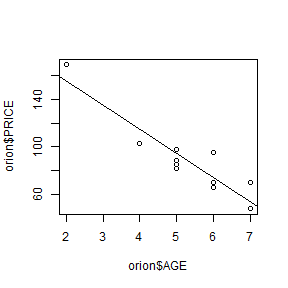
\includegraphics[width=\maxwidth]{figure/ex14-06} 

\end{knitrout}

%example 14.7
\subsection{Introduces the Coefficient of Determination}

\begin{knitrout}
\definecolor{shadecolor}{rgb}{0.969, 0.969, 0.969}\color{fgcolor}\begin{kframe}
\begin{alltt}
\hlcom{# load Orion data}
\hlstd{orion} \hlkwb{<-} \hlkwd{read.csv}\hlstd{(}\hlstr{"data/Tb14-02.txt"}\hlstd{,} \hlkwc{sep} \hlstd{=} \hlstr{"\textbackslash{}t"}\hlstd{)}
\hlkwd{str}\hlstd{(orion)}
\end{alltt}
\begin{verbatim}
## 'data.frame':	11 obs. of  2 variables:
##  $ AGE  : int  5 4 6 5 5 5 6 6 2 7 ...
##  $ PRICE: int  85 103 70 82 89 98 66 95 169 70 ...
\end{verbatim}
\begin{alltt}
\hlstd{y.sub.ybar} \hlkwb{<-} \hlstd{orion}\hlopt{$}\hlstd{PRICE} \hlopt{-} \hlkwd{mean}\hlstd{(orion}\hlopt{$}\hlstd{PRICE)}
\hlstd{y.sub.ybar}
\end{alltt}
\begin{verbatim}
##  [1]  -3.6364  14.3636 -18.6364  -6.6364   0.3636   9.3636 -22.6364
##  [8]   6.3636  80.3636 -18.6364 -40.6364
\end{verbatim}
\begin{alltt}
\hlstd{y.sub.ybar.sqr} \hlkwb{<-} \hlstd{y.sub.ybar}\hlopt{^}\hlnum{2}
\hlstd{y.sub.ybar.sqr}
\end{alltt}
\begin{verbatim}
##  [1]   13.2231  206.3140  347.3140   44.0413    0.1322   87.6777  512.4050
##  [8]   40.4959 6458.3140  347.3140 1651.3140
\end{verbatim}
\begin{alltt}
\hlstd{t} \hlkwb{<-} \hlkwd{data.frame}\hlstd{(orion,y.sub.ybar,y.sub.ybar.sqr)}
\hlstd{s} \hlkwb{<-} \hlkwd{lm}\hlstd{(orion}\hlopt{$}\hlstd{PRICE} \hlopt{~} \hlstd{orion}\hlopt{$}\hlstd{AGE)}
\hlstd{yhat} \hlkwb{<-} \hlstd{s}\hlopt{$}\hlstd{coefficients[[}\hlnum{1}\hlstd{]]} \hlopt{+} \hlstd{(s}\hlopt{$}\hlstd{coefficients[[}\hlnum{2}\hlstd{]]} \hlopt{*} \hlstd{t}\hlopt{$}\hlstd{AGE)}
\hlstd{t}\hlopt{$}\hlstd{yhat} \hlkwb{<-} \hlstd{yhat}
\hlstd{yhat.sub.ybar} \hlkwb{<-} \hlstd{t}\hlopt{$}\hlstd{yhat} \hlopt{-} \hlkwd{mean}\hlstd{(t}\hlopt{$}\hlstd{PRICE)}
\hlstd{t}\hlopt{$}\hlstd{yhat.sub.ybar} \hlkwb{<-} \hlstd{yhat.sub.ybar}
\hlstd{y.sub.yhat.sqr} \hlkwb{<-} \hlstd{(t}\hlopt{$}\hlstd{PRICE} \hlopt{-} \hlstd{t}\hlopt{$}\hlstd{yhat)}\hlopt{^}\hlnum{2}
\hlstd{t}\hlopt{$}\hlstd{y.sub.yhat.sqr} \hlkwb{<-} \hlstd{y.sub.yhat.sqr}
\hlstd{yhat.sub.ybar.sqr} \hlkwb{<-} \hlstd{(yhat} \hlopt{-} \hlkwd{mean}\hlstd{(t}\hlopt{$}\hlstd{PRICE))}\hlopt{^}\hlnum{2}
\hlstd{t}\hlopt{$}\hlstd{yhat.sub.ybar.sqr} \hlkwb{<-} \hlstd{yhat.sub.ybar.sqr}
\hlstd{t}
\end{alltt}
\begin{verbatim}
##    AGE PRICE y.sub.ybar y.sub.ybar.sqr   yhat yhat.sub.ybar y.sub.yhat.sqr
## 1    5    85    -3.6364        13.2231  94.16         5.526          83.95
## 2    4   103    14.3636       206.3140 114.42        25.787         130.49
## 3    6    70   -18.6364       347.3140  73.90       -14.735          15.22
## 4    5    82    -6.6364        44.0413  94.16         5.526         147.92
## 5    5    89     0.3636         0.1322  94.16         5.526          26.65
## 6    5    98     9.3636        87.6777  94.16         5.526          14.73
## 7    6    66   -22.6364       512.4050  73.90       -14.735          62.42
## 8    6    95     6.3636        40.4959  73.90       -14.735         445.17
## 9    2   169    80.3636      6458.3140 154.95        66.310         197.52
## 10   7    70   -18.6364       347.3140  53.64       -34.997         267.66
## 11   7    48   -40.6364      1651.3140  53.64       -34.997          31.81
##    yhat.sub.ybar.sqr
## 1              30.53
## 2             664.97
## 3             217.13
## 4              30.53
## 5              30.53
## 6              30.53
## 7             217.13
## 8             217.13
## 9            4396.96
## 10           1224.77
## 11           1224.77
\end{verbatim}
\begin{alltt}
\hlstd{sst} \hlkwb{<-} \hlkwd{sum}\hlstd{(t}\hlopt{$}\hlstd{y.sub.ybar.sqr)}
\hlstd{sst}
\end{alltt}
\begin{verbatim}
## [1] 9709
\end{verbatim}
\begin{alltt}
\hlstd{ssr} \hlkwb{<-} \hlkwd{sum}\hlstd{((t}\hlopt{$}\hlstd{yhat} \hlopt{-} \hlkwd{mean}\hlstd{(t}\hlopt{$}\hlstd{PRICE))}\hlopt{^}\hlnum{2}\hlstd{)}
\hlstd{ssr}
\end{alltt}
\begin{verbatim}
## [1] 8285
\end{verbatim}
\begin{alltt}
\hlstd{r.sqrd} \hlkwb{<-} \hlstd{ssr} \hlopt{/} \hlstd{sst}
\hlstd{r.sqrd}
\end{alltt}
\begin{verbatim}
## [1] 0.8534
\end{verbatim}
\begin{alltt}
\hlstd{sse} \hlkwb{<-} \hlkwd{sum}\hlstd{((t}\hlopt{$}\hlstd{PRICE} \hlopt{-} \hlstd{t}\hlopt{$}\hlstd{yhat)}\hlopt{^}\hlnum{2}\hlstd{)}
\hlstd{sse}
\end{alltt}
\begin{verbatim}
## [1] 1424
\end{verbatim}
\end{kframe}
\end{knitrout}

%example 14.8
\subsection{Computing Formulas for the Sum of Squares}

\begin{knitrout}
\definecolor{shadecolor}{rgb}{0.969, 0.969, 0.969}\color{fgcolor}\begin{kframe}
\begin{alltt}
\hlcom{# load Orion data}
\hlstd{orion} \hlkwb{<-} \hlkwd{read.csv}\hlstd{(}\hlstr{"data/Tb14-02.txt"}\hlstd{,} \hlkwc{sep} \hlstd{=} \hlstr{"\textbackslash{}t"}\hlstd{)}
\hlkwd{str}\hlstd{(orion)}
\end{alltt}
\begin{verbatim}
## 'data.frame':	11 obs. of  2 variables:
##  $ AGE  : int  5 4 6 5 5 5 6 6 2 7 ...
##  $ PRICE: int  85 103 70 82 89 98 66 95 169 70 ...
\end{verbatim}
\begin{alltt}
\hlstd{xx} \hlkwb{<-} \hlstd{orion}\hlopt{$}\hlstd{AGE}\hlopt{^}\hlnum{2}
\hlstd{yy} \hlkwb{<-} \hlstd{orion}\hlopt{$}\hlstd{PRICE}\hlopt{^}\hlnum{2}
\hlstd{xy} \hlkwb{<-} \hlstd{orion}\hlopt{$}\hlstd{AGE} \hlopt{*} \hlstd{orion}\hlopt{$}\hlstd{PRICE}
\hlstd{t} \hlkwb{<-} \hlkwd{data.frame}\hlstd{(orion, xx, yy, xy)}
\hlstd{t}
\end{alltt}
\begin{verbatim}
##    AGE PRICE xx    yy  xy
## 1    5    85 25  7225 425
## 2    4   103 16 10609 412
## 3    6    70 36  4900 420
## 4    5    82 25  6724 410
## 5    5    89 25  7921 445
## 6    5    98 25  9604 490
## 7    6    66 36  4356 396
## 8    6    95 36  9025 570
## 9    2   169  4 28561 338
## 10   7    70 49  4900 490
## 11   7    48 49  2304 336
\end{verbatim}
\begin{alltt}
\hlstd{sum.x} \hlkwb{<-} \hlkwd{sum}\hlstd{(t}\hlopt{$}\hlstd{AGE)}
\hlstd{sum.y} \hlkwb{<-} \hlkwd{sum}\hlstd{(t}\hlopt{$}\hlstd{PRICE)}
\hlstd{sum.xx} \hlkwb{<-} \hlkwd{sum}\hlstd{(t}\hlopt{$}\hlstd{xx)}
\hlstd{sum.yy} \hlkwb{<-} \hlkwd{sum}\hlstd{(t}\hlopt{$}\hlstd{yy)}
\hlstd{sum.xy} \hlkwb{<-} \hlkwd{sum}\hlstd{(t}\hlopt{$}\hlstd{xy)}
\hlstd{sst} \hlkwb{<-} \hlstd{sum.yy} \hlopt{-} \hlstd{(sum.y}\hlopt{^}\hlnum{2} \hlopt{/} \hlkwd{nrow}\hlstd{(t))}
\hlstd{sst}
\end{alltt}
\begin{verbatim}
## [1] 9709
\end{verbatim}
\begin{alltt}
\hlstd{num} \hlkwb{<-} \hlstd{(sum.xy} \hlopt{-} \hlstd{(sum.x} \hlopt{*} \hlstd{sum.y} \hlopt{/} \hlkwd{nrow}\hlstd{(t)))}\hlopt{^}\hlnum{2}
\hlstd{den} \hlkwb{<-} \hlstd{sum.xx} \hlopt{-} \hlstd{sum.x}\hlopt{^}\hlnum{2} \hlopt{/} \hlkwd{nrow}\hlstd{(t)}
\hlstd{ssr} \hlkwb{<-} \hlstd{num} \hlopt{/} \hlstd{den}
\hlstd{ssr}
\end{alltt}
\begin{verbatim}
## [1] 8285
\end{verbatim}
\begin{alltt}
\hlstd{sse} \hlkwb{<-} \hlstd{sst} \hlopt{-} \hlstd{ssr}
\hlstd{sse}
\end{alltt}
\begin{verbatim}
## [1] 1424
\end{verbatim}
\end{kframe}
\end{knitrout}

%example 14.9
\subsection{Using Technology to Obtain a Coefficient of Determination}

\begin{knitrout}
\definecolor{shadecolor}{rgb}{0.969, 0.969, 0.969}\color{fgcolor}\begin{kframe}
\begin{alltt}
\hlcom{# read in the data}
\hlstd{orion} \hlkwb{<-} \hlkwd{read.csv}\hlstd{(}\hlstr{"data/Tb14-02.txt"}\hlstd{,} \hlkwc{sep} \hlstd{=} \hlstr{"\textbackslash{}t"}\hlstd{)}
\hlkwd{str}\hlstd{(orion)}
\end{alltt}
\begin{verbatim}
## 'data.frame':	11 obs. of  2 variables:
##  $ AGE  : int  5 4 6 5 5 5 6 6 2 7 ...
##  $ PRICE: int  85 103 70 82 89 98 66 95 169 70 ...
\end{verbatim}
\begin{alltt}
\hlstd{s} \hlkwb{<-} \hlkwd{lm}\hlstd{(orion}\hlopt{$}\hlstd{PRICE} \hlopt{~} \hlstd{orion}\hlopt{$}\hlstd{AGE)}
\hlkwd{summary}\hlstd{(s)}
\end{alltt}
\begin{verbatim}
## 
## Call:
## lm(formula = orion$PRICE ~ orion$AGE)
## 
## Residuals:
##    Min     1Q Median     3Q    Max 
## -12.16  -8.53  -5.16   8.95  21.10 
## 
## Coefficients:
##             Estimate Std. Error t value Pr(>|t|)    
## (Intercept)    195.5       15.2   12.83  4.4e-07 ***
## orion$AGE      -20.3        2.8   -7.24  4.9e-05 ***
## ---
## Signif. codes:  0 '***' 0.001 '**' 0.01 '*' 0.05 '.' 0.1 ' ' 1
## 
## Residual standard error: 12.6 on 9 degrees of freedom
## Multiple R-squared:  0.853,	Adjusted R-squared:  0.837 
## F-statistic: 52.4 on 1 and 9 DF,  p-value: 4.88e-05
\end{verbatim}
\begin{alltt}
\hlkwd{summary}\hlstd{(s)}\hlopt{$}\hlstd{r.squared}
\end{alltt}
\begin{verbatim}
## [1] 0.8534
\end{verbatim}
\end{kframe}
\end{knitrout}

%example 14.10
\subsection{}



%example 14.11
\subsection{}



%chapter 15
\section{Inferential Methods in Regression and Correlation}
%chapter 16
\section{Analysis of Variance (ANOVA)}



\end{document}
